\documentclass{article}
\usepackage{../../Self_Style}

\title{Phys 20BL Week 4 Out of Lab: Speed of Sound}
\author{Zih-Yu Hsieh}
\date{\today}

\begin{document}
\maketitle

\tableofcontents

\newpage

\section{Model of Fluid for Sound Propogation}
\subsection{Model Derivation}
First, it's assumed that the speed is given as:
\begin{align}
    v=\sqrt{\frac{B}{\rho}}
\end{align}
Where $B$ is the Bulk Modulus (the resistance against compression of the material), while $\rho$ is the density. 

This intuitively follows from the observation that in a relatively incompressable fluid (for instance, water vs. air), the speed is traveling faster; on the other hand, the increase in density increases the amount of material the wave needs to propogate through, which naively explains the decrease in speed.

\hfil

Then, therelation of Bulk Modulus is proportional to the pressure when assuming the gas is an ideal gas:
\begin{align}
    B=\gamma P
\end{align}
Where $\gamma$ is the heat ratio of gas, called Adiabatic Index. 

\hfil

Also, with the assumption of the gas being an ideal gas, one applies the ideal gas law:
\begin{align}
    PV = N k_B T
\end{align}
Where $V$ is the gas volume, $N$ is the number of gas molecules, $k_B$ is the Boltzmann constant, and $T$ is the temperature in Kelvin.

With these variables, the density of the gas can be given as follow:
\begin{align}
    \rho = \frac{N m}{V}
\end{align}
Since if $m$ represents the average msas of molecules (mass of ``unit volume''), then $N m$ represents the total mass of the occupied volume; hence, dividing by the total volume, one recovers the density.

\hfil

By plugging in all the terms from the other equations to the first one (and using the extra derivation $\frac{N}{V}=\frac{P}{k_B T}$ by ideal gas law), one yields the following derivation:
\begin{align}
    v = \sqrt{\frac{B}{\rho}}=\sqrt{\frac{\gamma P}{Nm/V}}= \sqrt{\frac{\gamma P}{Pm/(k_B T)}} = \sqrt{\frac{\gamma k_B T}{m}}
\end{align}

\hfil

\subsection{Assumptions of the Model}
The first assumption of the model is that the gas must be ideal gas (which under this experiment without extreme compression, it'll be a suitable approximation).

On the other hand, it's also assumed that the Bulk Modulus is always proportional to the pressure of  the gas $P$.

\newpage

\section{Model Prediction of Speed of Sound}
\subsection{Constant Values}
First, here are some given cconstants: $k_B := 1.380649 \cdot 10^{-23}$ J$\cdot$K$^{-1}$, while $\gamma:= 1.4$.

\hfil

For temperature, the weather report at Goleta during the time of experiment is used, which provides $T = 16^\circ$C $= 289.15$ K. In this lab, because the equipment used to observe environmental temperature / humidity / CO$_2$ concentration are all broken (or non-existent), one needs external sources for the data.
\begin{figure}[h!]
    \centering
    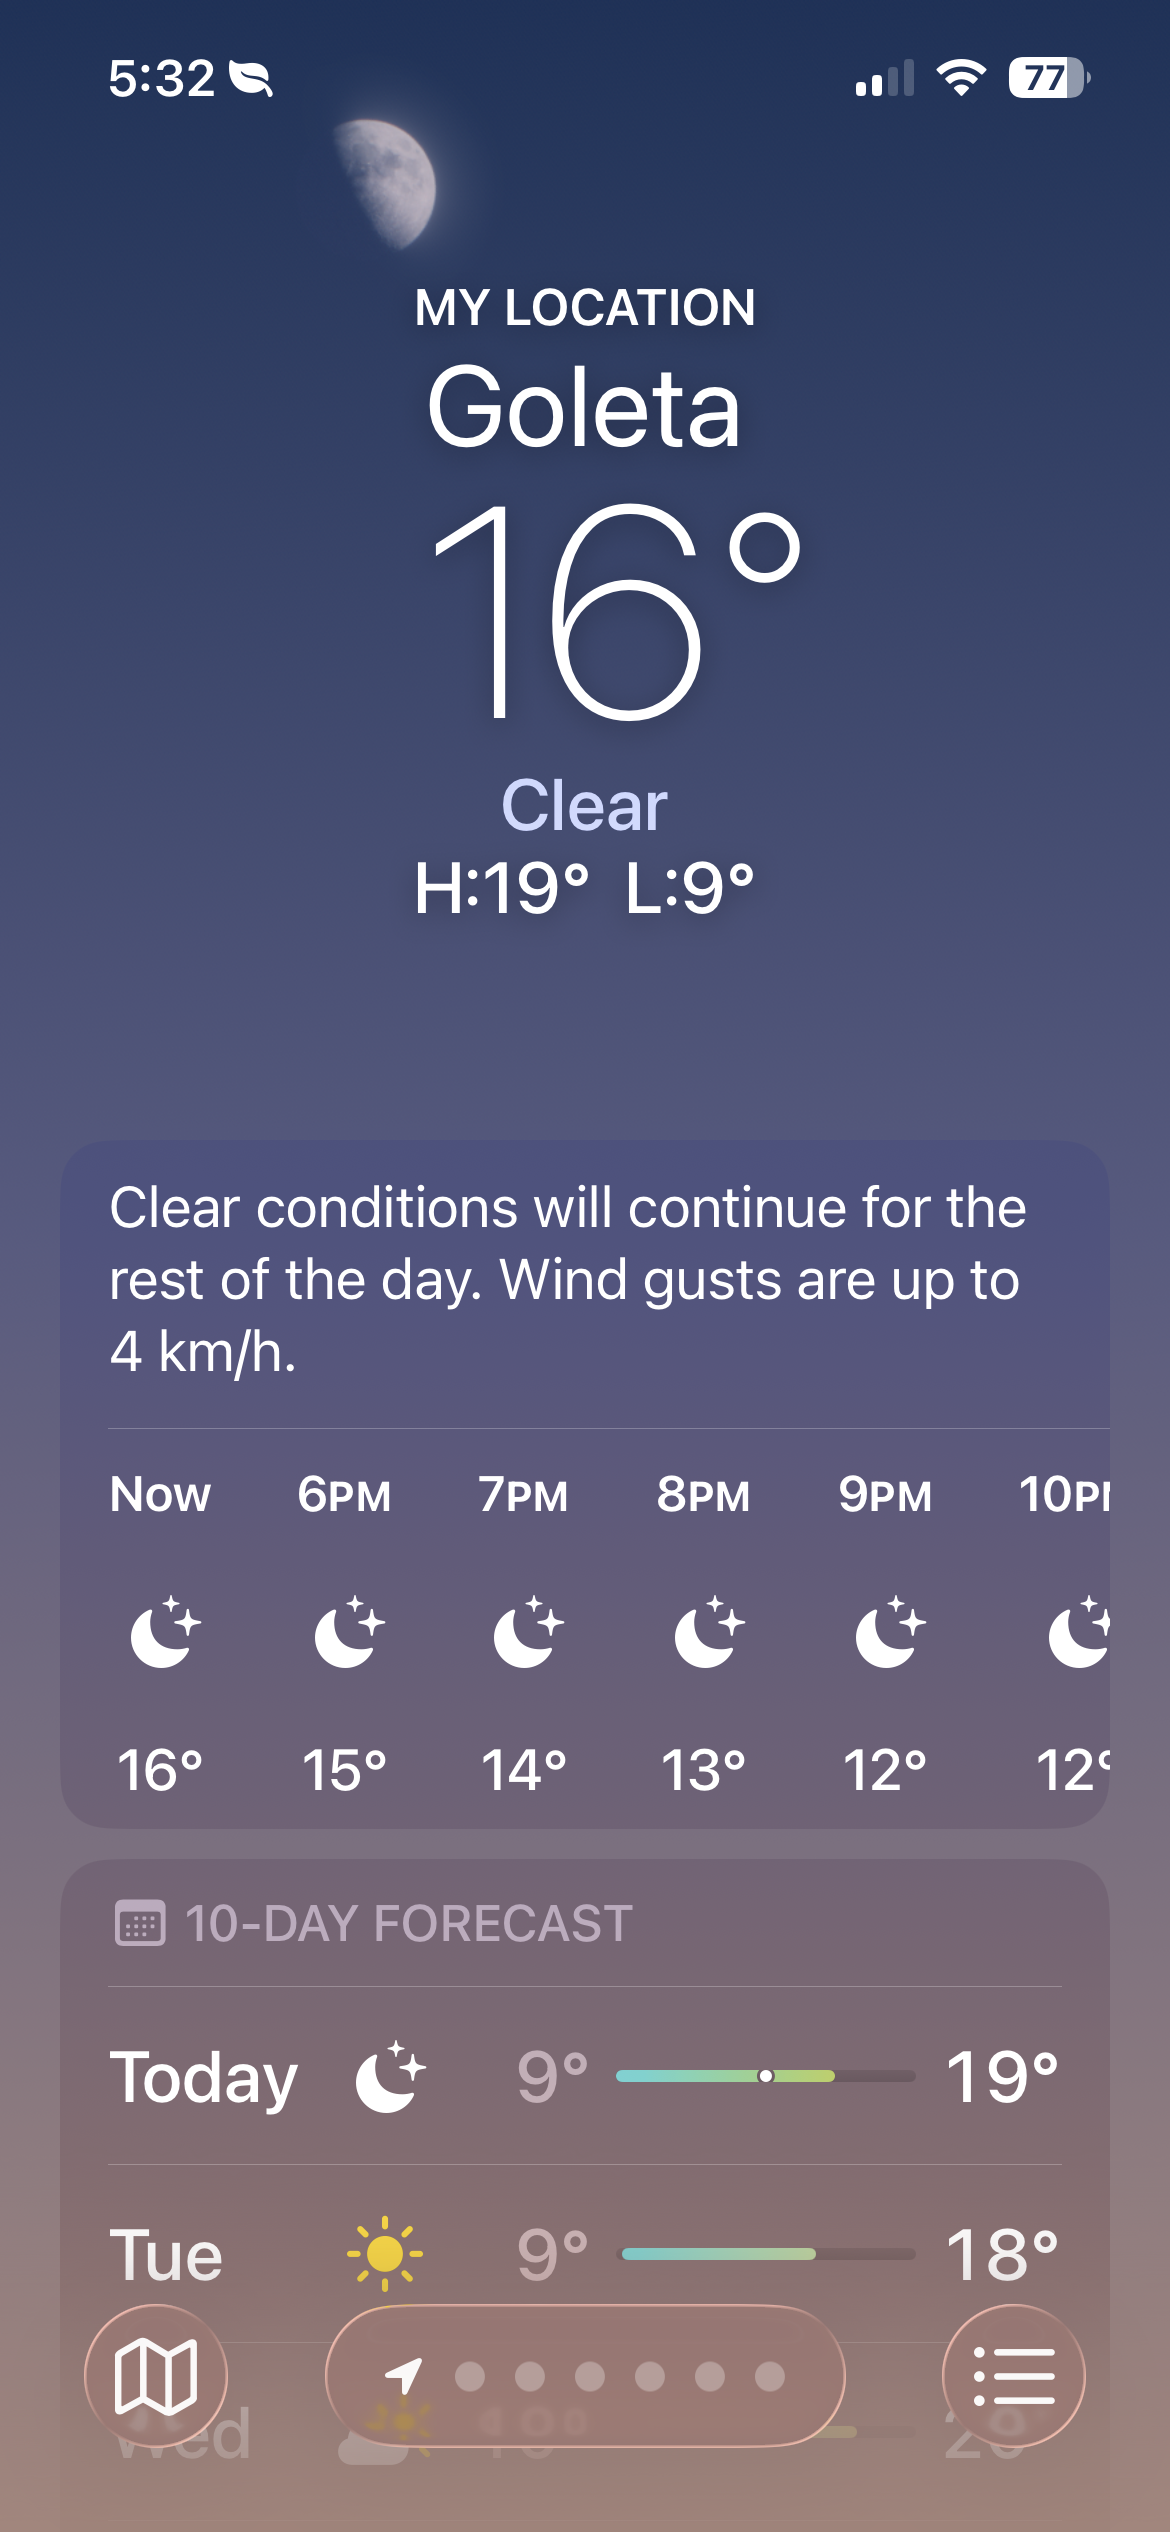
\includegraphics[width=40mm]{temperature.png}
    \caption{A screenshot of the temperature during the lab (Monday, January 26, 2026)}
\end{figure}

\hfil

For the molecular gas mass, we'll accept the value $m \approx 4.81\cdot 10^{-26}$ kg, which is derived from the weighted average of the masses of the common gases based on their percentage within the atmosphere. The molecular gas masses of the common gases, are found on the National Institute of Standards and Technology website.

(Source: National Institute of Standards and Technology, ``Search for Species Data by Molecular Weight''.https://webbook.nist.gov/chemistry/mw-ser/)

\hfil

\subsection{Sources of Deviation in $\gamma$}
If consider the potential inaccuracy of $\gamma$, the humidity of the day may be a potential source of error: As the air gets more humid, the water molecules in it would increase the overall mass of the gas, hence increasing the density. Yet, the constant $\gamma$ is also related to the density by the formula $B = \rho\frac{dP}{d\rho}$. Which, with the lab day being somewhat humid, the constant $\gamma$ might not accurately be $1.4$.

\hfil

\subsection{Uncertainties}
For $k_B$ the Boltzmann constant, the uncertainty is assumed to be $0$ (since according to the instruction one can believe it's near an exact value). For $\gamma$, one could suppose $\delta \gamma=\pm 0.05$ (since the given value is up to the $10$th decimal place, which the error by $0.05$ is not possible to verify). Finally, for the temperature, one has $\delta T = \pm 0.5$ K (since the temperature given by the weath report is always in integer values of unit Celcius,so an error of $0.5$ K is not possible to be observed).

\hfil

\subsection{Proposed Speed of Sound}
Given the values, one has the following value for the speed of sound:
\begin{align}
    v=\sqrt{\frac{\gamma k_B T}{m}} = \sqrt{\frac{1.4\cdot 1.380649\cdot 10^{-23}\cdot 289.15}{4.81\cdot 10^{-26}}} \approx 340.875 \text{ m/s}
\end{align}
Which, the unit of the middle expression is $\sqrt{\frac{\text{J}}{\text{kg}}}=\sqrt{\frac{\text{kg}\cdot\text{m}^2\text{/s}^2}{\text{kg}}} = \sqrt{\frac{\text{m}^2}{\text{s}^2}} =$ m/s.

\hfil

\hfil

\section{Data Analysis}
For both approaches (with different sound frequency), we had gathered the average time difference and time difference uncertainty for each trial. Which, $D$ (unit: m) represents the distance of the microphone from the speaker, $t_i$ (unit: ms) represents the average time difference between the original and the received signal in the $i$th trial.

\hfil

\subsection{Frequency $f=1$ kHz}

The data is given in the following table:
\begin{table}[h]
\centering
\begin{tabular}{|cc||c c||cc||cc|}
\hline
\multicolumn{2}{|c|}{Distance (m)} & \multicolumn{6}{c|}{Time (ms)} \\
\hline
$D$ & $\delta D$ & $t_1$ & $\delta t_1$ & $t_2$ & $\delta t_2$ & $t_3$ & $\delta t_3$ \\
\hline
0.81 & 0.0005 & 3.3133 & 0.0231 & 3.3400 & 0.0200 & 3.3400 & 0.0000 \\
1.01 & 0.0005 & 2.7667 & 0.0115 & 2.7467 & 0.0115 & 2.7533 & 0.0115 \\
1.21 & 0.0005 & 2.1867 & 0.0115 & 2.1933 & 0.0115 & 2.1867 & 0.0115 \\
\hline
\end{tabular}
\label{tab:distance_time}
\end{table}
When making into scatter plot, one yields the following:
\begin{figure}
    \centering
    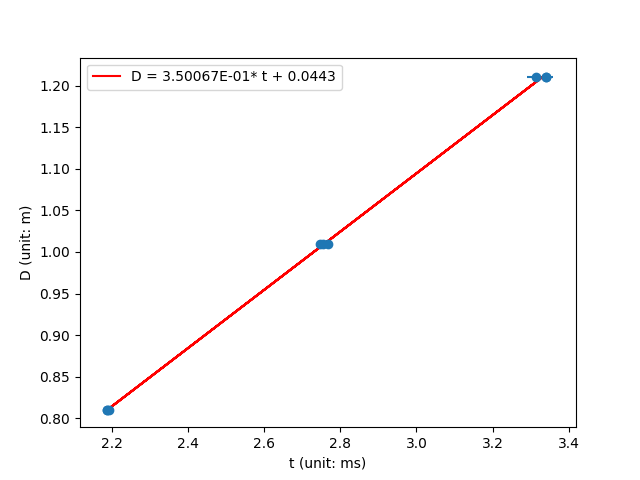
\includegraphics[width=100mm]{scatter_plot_1.png}
\end{figure}

\newpage

So, the best-fitting line for the data is given as follow:
\begin{align}
    D = 3.50067\cdot 10^{-1}t+0.0443
\end{align}
Where $D$ is the distance the wave traveled (unit: m), and $t$ is the time it takes for the travel (unit: ms).

As a result, the best-fit speed of sound in air would be given by the slope of the best-fit line, which is $3.50067\cdot 10^{-1}$ m/ms, which translates to speed $v=350.0670$ m/s.

\hfil

\subsection{Frequency $f=1.25$ kHz}
The data is given in the following table:
\begin{table}[h]
\centering
\label{tab:distance_time_ms}
\begin{tabular}{|cc||cc||cc||cc|}
\hline
\multicolumn{2}{|c|}{Distance (m)} & \multicolumn{6}{c|}{Time (ms)} \\
\hline
$D$ & $\delta D$ 
& $t_1$ & $\delta t_1$
& $t_2$ & $\delta t_2$
& $t_3$ & $\delta t_3$ \\
\hline
1.21 & 0.0005 & 3.3600 & 0.0200 & 3.3800 & 0.0200 & 3.3800 & 0.0200 \\
1.01 & 0.0005 & 2.7867 & 0.0115 & 2.7533 & 0.0231 & 2.7800 & 0.0200 \\
0.81 & 0.0005 & 2.1867 & 0.0115 & 2.1933 & 0.0115 & 2.1933 & 0.0115 \\
\hline
\end{tabular}
\end{table}



\end{document}